\chapter{Results and Inferences}

This chapter looks at the various results of the simulations the models have gone through. It is shown that the system parameter, \acrshort{ber} is within the required limits (less than $10^{-5}$) and the report also discusses the time taken to transmit $10^6$ bits in the various schemes. Comparisons and contrasts are drawn between the results obtained across different schemes and conclusions are drawn.

\section{List of Simulations and their Parameters}
The list of various simulations and their parameters is given in \ref{List of Simulations and their Parameters}.\\

The common channel parameters for all simulations is as follows
\begin{itemize}
\item In all simulations the noise power spectral density is -80 dBm/Hz
\item The distance between the transmitting and receiving antenna is 1km
\item The gain of the \acrshort{bs} antenna is 8 and \acrshort{ue} antenna is taken as 1
\item The maximum number of bits that can be loaded on a subchannel in case of tone loading operation being performed at the transmitter is 20 bits.
\item The number of subchannels is taken to be 256.
\item The power input to the transmitter is 1 mW.
\end{itemize}

Apart from these there are certain randomized parameters such as the \gls{rayleigh fading} coefficient and the noise signal which is additive white Gaussian in nature.

\begin{table}[htpb]
\centering
\label{List of Simulations and their Parameters}
\caption{List of Simulations and Parameters}
\begin{tabular}{ |p{3cm}||p{3cm}|p{3cm}|p{3cm}| |p{3cm}|}
 \hline
 \multicolumn{5}{|c|}{Simulation Parameters} \\
 \hline
 Simulation Mode & Number of bits & Precoding Scheme & \acrshort{ber} & Number of cycles\\
 \hline
 SISO & $10^6$    & - &   0 & 1643\\
 SIMO & $10^6$    & Alamouti Precoding &   0 & 1051\\
 MISO & $10^6$    & - &   0 & 98\\
 MIMO & $10^6$    & Inverse Channel Estimation Precoding and Singular Value Decomposition Precoding &   0 & 98\\
 \hline
\end{tabular}
\end{table}

\section{SISO System Results}
The result for the \acrshort{siso} simulation is shown in figure \ref{fig:siso system performance}. The \acrshort{ber} is observed to be $0$, which is within the expected range. Also, the total power deviation due to rounding of the number of bits per tone is $-0.95131$ dB which is less than our threshold value of $\pm 2$ dB.\\
It is observed in figure \ref{fig:siso tone loading} that the subchannels with higher \acrshort{snr} have more bits loaded onto them which is the expected behavior of our tone loading algorithm.\\
\textbf{Inference:}\\
Since there is only one antenna path to transmit $10^6$ bits, there is a need of a total of $1643$ cycles of transmitting bits as per the tone loading profile in \ref{fig:siso tone loading}. Due to the lack of multiple antenna paths, it takes a long time to transmit the bits. To improve the speed (data rate), one must either improve the \acrshort{snr} of the channel to improve the channel capacity or go for \acrshort{mcm}-\acrshort{mimo} system. Since the first option is not in our control, it is discussed in the future sections how \acrshort{mcm}-\acrshort{mimo} can improve the data rates and capacity.

\begin{figure}[!htbp]
\centering
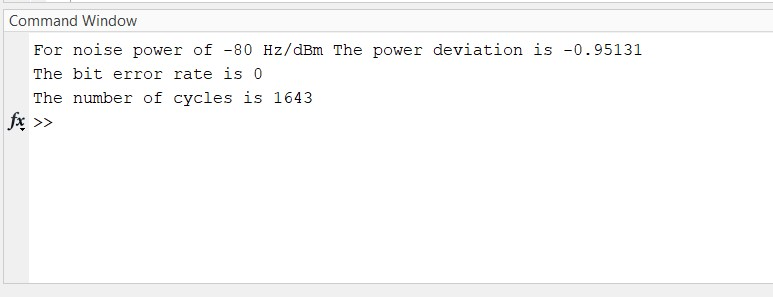
\includegraphics[scale=1]{Chapter 4/Figures/SISO System Performance}
\caption[SISO Tone Loading]{The performance of our SISO system. The number of cycles taken to transmit the bits is of particular importance to us. }
\label{fig:siso system performance}
\end{figure}

\begin{figure}[!htbp]
\centering
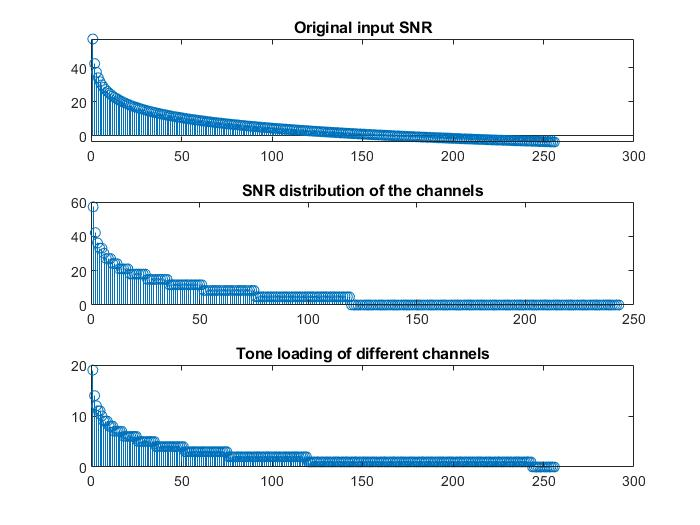
\includegraphics[scale=0.7]{Chapter 4/Figures/SISO Tone Loading}
\caption[SISO Tone Loading]{The tone loading profile of various subchannels for SISO mode.}
\label{fig:siso tone loading}
\end{figure}

\section{SIMO System Results}
The result for the \acrshort{simo} simulation is shown in figure \ref{fig:simo system performance}. The \acrshort{ber} is observed to be $0$, which is within the expected range. Also, the total power deviation due to rounding of the number of bits per tone is $-1.82$ dB which is less than our threshold value of $\pm 2$ dB.\\
It is observed in figure \ref{fig:simo tone loading} that the subchannels with higher \acrshort{snr} have more bits loaded onto them which is the expected behavior of our tone loading algorithm.\\

\textbf{Inference:}\\
To transmit $10^6$ bits, one needs a total of $1051$ cycles of transmitting bits as per the tone loading profile in \ref{fig:simo tone loading}. This case is also known as receiver diversity, wherein one chooses the best path between the transmitter and receiver and use that path for the transmission of data. By periodically checking for the best path, it is possible to maintain a good quality link between transmitter and receiver that despite bad channel conditions.

\begin{figure}[!htbp]
\centering
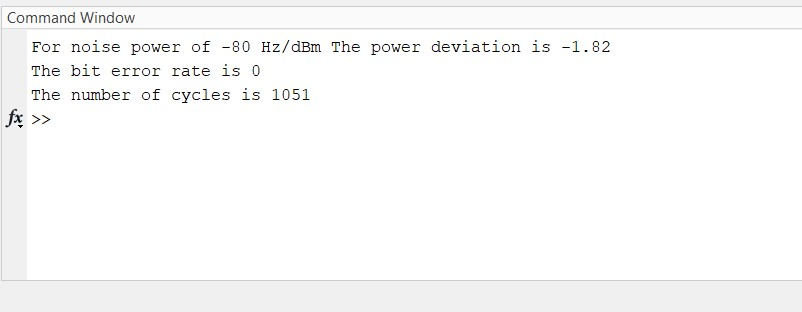
\includegraphics[scale=1]{Chapter 4/Figures/SIMO System Performance}
\caption[SIMO Tone Loading]{The performance of our SIMO system. The number of cycles taken to transmit the bits is of particular importance to us.}
\label{fig:simo system performance}
\end{figure}

\begin{figure}[!htbp]
\centering
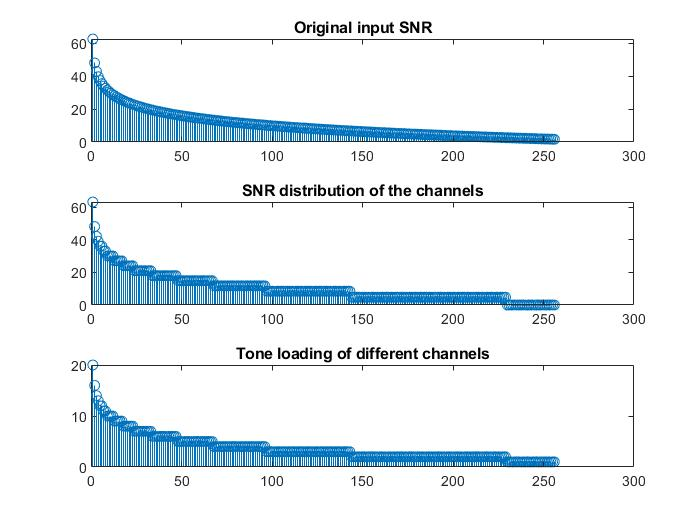
\includegraphics[scale=0.7]{Chapter 4/Figures/SIMO Tone Loading}
\caption[SIMO Tone Loading]{The tone loading profile of various subchannels for SIMO mode.}
\label{fig:simo tone loading}
\end{figure}

\section{MISO System Results}
The result for the \acrshort{miso} simulation is shown in the figure \ref{fig:miso system performance}. The \acrshort{ber} is observed to be $0$, which is within the expected range. One need not perform any tone loading as Alamouti precoding scheme is used. 

\textbf{Inference:}\\
It takes only $98$ cycles to transmit the $10^6$ bits. Since there are multiple transmitting antennas that use Alamouti coding, one is able to send 2 symbols in 2 time intervals, however with increase in the number of antennas the efficiency of the precoding falls. One can use this system to accommodate 2 sets of symbols from the same user thus improving the data rate or symbols from 2 different users thus improving the capacity of the system.


\begin{figure}[!htbp]
\centering
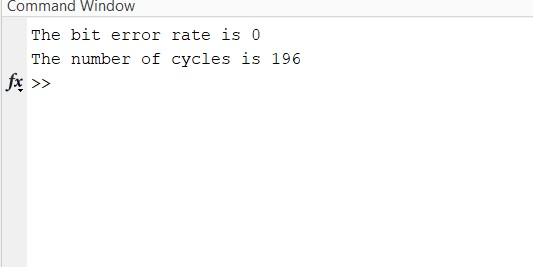
\includegraphics[scale=1]{Chapter 4/Figures/MISO System Performance}
\caption{MISO System Performance.}
\label{fig:miso system performance}
\end{figure}

\section{MIMO System Results}

\subsection{MIMO Diversity Case}
The result for the \acrshort{mimo} simulation in diversity case is shown in figure \ref{fig:mimo system performance diversity}. The \acrshort{ber} is observed to be $0$, which is within the expected range. Also, the total power deviation due to rounding of the number of bits per tone is $-1.3892$ dB which is less than our threshold value of $\pm 2$ dB.\\
It is observed in figure \ref{fig:mimo tone loading diversity} that the subchannels with higher \acrshort{snr} have more bits loaded onto them which is the expected behavior of our tone loading algorithm. One needs a total of $1303$ cycles of transmitting bits as per the tone loading profile in \ref{fig:mimo tone loading diversity}\\

\textbf{Interference:}\\
Although one has many antenna paths to transmit $10^6$ bits, since one is operating in diversity mode, the system is only using the best channel between these two to transmit our data, hence one does not seeing much improvement in speed. It is seen how operating \acrshort{mimo} in multiplexing mode can vastly improve this system performance.

\begin{figure}[!htbp]
\centering
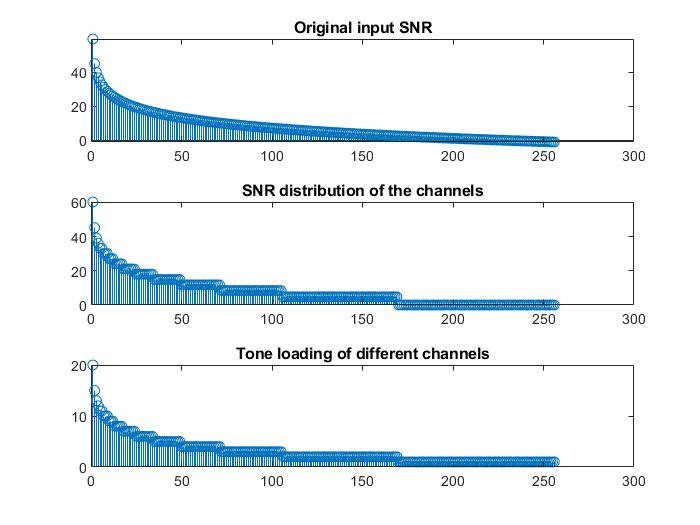
\includegraphics[scale=0.7]{Chapter 4/Figures/MIMO Tone Loading Diversity}
\caption[MIMO Tone Loading in Diversity Case]{The tone loading profile of various subchannels for MIMO in diversity mode.}
\label{fig:mimo tone loading diversity}
\end{figure}

\begin{figure}[!htbp]
\centering
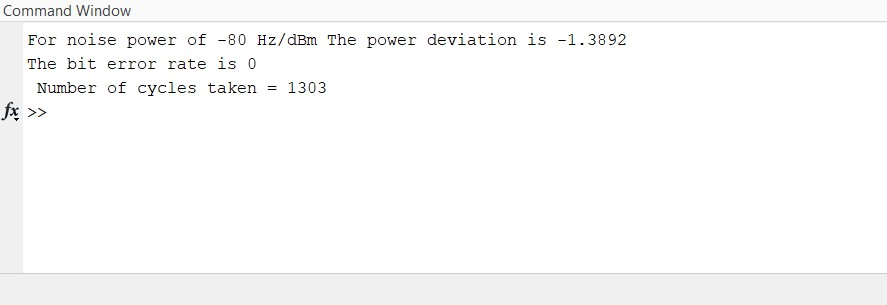
\includegraphics[scale=1]{Chapter 4/Figures/MIMO System Performance Diversity}
\caption[MIMO System Performance in Diversity Case]{The performance of our MIMO system. The number of cycles taken to transmit the bits is of particular importance to us.}
\label{fig:mimo system performance diversity}
\end{figure}

\subsection{MIMO Multiplexing with Inverse Channel Estimation Precoder}

The result for the \acrshort{mimo} simulation for multiplexing case with inverse channel estimation precoder is shown in the figure \ref{fig:mimo system performance inverse channel estimation}. The \acrshort{ber} is observed to be $0$, which is within the expected range. There is no need to perform any tone loading as the system uses a Inverse Channel Estimation precoding scheme.\\

\textbf{Inference:}\\
It takes only $98$ cycles to transmit the $10^6$ bits. One notices how by using suitable precoding the number of cycles reduce drastically. Since the system is using Inverse Channel Estimation precoding, there is no need for a decoder at the receiver as the channel effects itself nullify the effect of the precoding. By using multiple antenna paths, data rates and capacities are vastly improved.

\begin{figure}[!htbp]
\centering
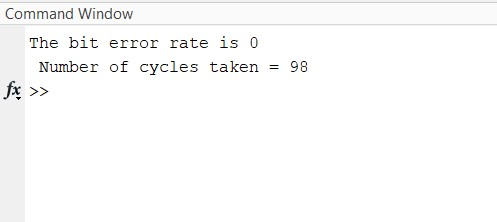
\includegraphics[scale=1]{Chapter 4/Figures/MIMO System Performance Inverse Channel Estimation}
\caption{MIMO System Performance with Inverse Channel Estimation Precoder.}
\label{fig:mimo system performance inverse channel estimation}
\end{figure}

\subsection{MIMO Multiplexing with Singular Value Decomposition Precoder}

The result for the \acrshort{mimo} simulation for multiplexing case with singular value decomposition precoder is shown in the figure \ref{fig:mimo system performance singular value decomposition}. The \acrshort{ber} is observed to be $0$, which is within the expected range. One does not perform any tone loading as the system uses a Singular Value Decomposition precoding scheme. It takes only $98$ cycles to transmit the $10^6$ bits. It is noticed how by using suitable precoding the number of cycles reduce drastically.\\

\textbf{Inference:}\\
Although the speed of \acrshort{svd} decomposition precoding is similar to that of Inverse Channel Estimation precoding, the speed of execution is noticed to be faster because it is computationally simpler to find the \acrshort{svd} of the matrix than to invert it. This is especially true when the size of the matrix is much larger than $2 \times 2$.

\begin{figure}[!htbp]
\centering
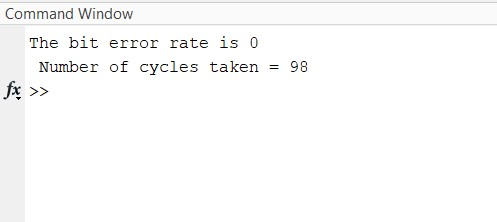
\includegraphics[scale=1]{Chapter 4/Figures/MIMO System Performance Inverse Channel Estimation}
\caption{MIMO System Performance with Singular Value Decomposition Precoder.}
\label{fig:mimo system performance singular value decomposition}
\end{figure}

\section*{Summary}
In this chapter the results of the simulations of our system in various configurations was discussed. Readers clearly see that data rates increase with multiplexing mode and also with precoding. Finally, in the last section the report is concluded and the future scope of the report is discussed and how further improvements can be made to our system is also mentioned.




